\graphicspath{{Dissertation/images/chapt3/}}

\chapter{Экстремальные яркостные температуры в обзоре активных ядер галактик} \label{chapt3}

\section{Яркостная температура}

\section{Обзор активных ядер галактик в проекте <<РадиоАстрон>>}


\section{RELATIVISTIC JETS IN THE RADIO REFERENCE FRAME IMAGE DATABASE. II. BLAZAR JET
ACCELERATIONS FROM THE FIRST 10 YEARS OF DATA (1994--2003)}
% \section{Измерение доплеровского усиления с помощью кинематики релятивистских струй}

\subsection{Введение}

Объемный отток вещества при высоких факторах Лоренца в коллимированных релятивистских струях
является хорошо известным свойством мощных блазаров. Такие высокие факторы Лоренца можно
непосредственно наблюдать по видимому движению высокоскоростных компонентов струи на изображениях,
построенных с помощью  интерферометрии со сверхдлинными базами (РСДБ) \cite{Lister_2009b}, и они
также необходимы для объяснения спектрального распределения энергии блазаров \cite{Hartman_2001},
переменности гамма-излучения \cite{Dondi_1995} и высокой яркостной температуры радио-ядра
\cite{Tingay_2001}. Эти релятивистские джеты должны ускорятся на масштабах расстояний от примерно
$10^3$ гравитационных радиусов от центральной черной дыры и до парсеков, где они непосредственно
наблюдаются с помощью РСДБ \cite{Sikora_2005,Vlahakis_2004}. Хотя наблюдения за потоками с высоким
фактором Лоренца хорошо установлены, теоретический механизм, с помощью которого эти потоки
ускоряются, и масштаб длины, на котором они работают, до конца не поняты.

В общем контексте ускорения магнитной струи в блазарах \cite{Sikora_2005} энергия потока начинается
как магнитная энергия, или поток вектора Пойнтинга, который затем преобразуется в объемную
кинетическую энергию во время фазы ускорения и, наконец, в кинетическую энергию частиц при ударах,
которая затем может излучиться. Магнитное ускорение было исследовано с помощью релятивистского
магнитогидродинамического моделирования (например \cite{McKinney_2006}; также см.
\cite{Komissarov_2011,Konigl_2010} для краткого описания теории магнитного ускорения релятивистских
струй).

Остается рассмотреть ряд деталей в этой общей структуре: например, создается ли струя в устойчивом
состоянии или ускорение является импульсным \cite{Granot_2011,Lyutikov_2010}, и
завершается ли ускорение на масштабах, наблюдаемых на РСДБ, или все еще происходит на
парсековых масштабах. В \cite{Vlahakis_2004} утверждается, что магнитное ускорение может
продолжать действовать в масштабах парсеков, и они интерпретировали два конкретных наблюдаемых
события ускорения в NGC\,6251 и 3C\,345 как свидетельство этого <<магнитного движения>> в
парсековых масштабах, но во времена той статьи было ещё недостаточно РСДБ наблюдений для
решения вопроса о том, является ли ускорение на масштабах парсеков общим свойством струй блазаров
на больших выборках. Даже если явление ускорения в масштабе парсек считается обычным явлением, это
не обязательно доказывает прямое наблюдение преобразования потока Пойнтинга в кинетическую энергию,
поскольку также могут быть гидродинамические механизмы для создания ускорений в джетах с
доминированием вещества \cite{Daly_1988,Kadler_2008}, или наблюдения могут
показывать увеличение факторов Лоренца структур в подстилающем потоке.

Прямые наблюдения внутреннего ускорения с помощью РСДБ картографирования затруднены. Точные
измерения положения компонентов на многих эпохах необходимы для надежного измерения второй
производной на графике положения от времени. Для отдельных компонентов струи кажущаяся скорость
определяется по известной формуле:

\[
 \beta_\text{app} = \frac{\beta \sin\theta}{1 - \beta \cos\theta}\,,
\]
\noindent
где $\beta c$~"--- собственная скорость, а $\theta$~"--- угол движения к лучу зрения. При
наблюдении в
одном компоненте изменения кажущейся скорости могут быть вызваны либо изменением собственной
скорости, либо угла обзора. Наблюдения за многими явно ускоряющимися компонентами необходимы для
статистического различия между этими двумя случаями. На практике, наблюдения за многими источниками
во многие эпохи, насчитывающие тысячи изображений РСДБ, необходимы для измерения вариаций
собственных скоростей. В то время как наблюдения за отдельными кажущимися ускорениями компонентов
(например, \cite{Unwin_1997,Homan_2003}) или видимых ускорений компонентов в небольших выборках
блазаров (например, \cite{Homan_2001,Jorstad_2005}) были ранее отмечены, обзор MOJAVE с 2424
изображениями был первым, в котором исследовались ускорения струй блазаров на большой статистической
выборке \cite{Homan_2009}.

В этой статье мы представляем продолжение нашего исследования кинематики струй блазаров,
проведенного в \cite{Piner_2007}, которое разработано для измерения ускорений в струях блазаров с
использованием серии экспериментов RDV (Research \& Development --- VLBA) на решетке апертурного
синтеза VLBA \cite{Petrov_2009}. Серия экспериментов RDV наблюдается в основном для целей
астрометрии и геодезии, но поскольку эксперименты проводятся примерно каждые два месяца с момента
открытия VLBA и дают качественные изображения, они также полезны для астрофизики блазаров (например,
\cite{Kovalev_2008,Pushkarev_2012b}). Это только второе крупномасштабное исследование ускорений
видимых движений внегалактических струй (после \cite{Homan_2009}).

В \cite{Piner_2007} мы анализировали кинематику струй, используя 19 РСДБ экспериментов,
наблюдавшихся в течение 5 лет с 1994 по 1998 год (RDV с 1 по 10 и 12, плюс 8 аналогичных РСДБ
экспериментов, которые были проведены на VLBA до начала серии RDV). В этой статье мы изучили
все источники, которые наблюдались в 3 или более эпохах за эти 19 экспериментов, в результате чего
было получено в общей сложности 966 изображений 87 источников, которые использовались для измерения
видимой скорости струй.

В этой статье мы расширим наше исследование из \cite{Piner_2007}, распространив анализ на 50 РСДБ
экспериментов за 10-летний период с 1994 по 2003 год (добавив 31 новый эксперимент RDV с 11 и 13 по
42) и изучив кинематику всех источников, которые наблюдались в 20 или более эпохах в этих 50
экспериментах. Этот обзор в дальнейшем именуется обзор RDV: в настоящее время он включает 2753 РСДБ
изображения 68 источников, с медианным значением 43 количества эпох наблюдения на источник.
Количество изображений приблизительно в три раза больше, чем в \cite{Piner_2007}, и немного
превышает 2424 изображения в обзоре MOJAVE \cite{Lister_2009a}. Отметим также, что максимальное
количество эпох на источник из \cite{Piner_2007} (19) теперь меньше, чем минимальное количество эпох
на источник, в этой статье (20).

Эксперименты RDV продолжались до настоящего времени; последний доступный на момент написания этой
статьи --- RDV 93, наблюдался 28 июня 2012 года. Таким образом, в архиве VLBA уже есть еще 51
эксперимент RDV, сверх того, что включено в эту статью. Если эти дополнительные эксперименты будут
полностью прокартографированы и отмоделированы, то они могут примерно вдвое увеличить размер
обзора RDV по сравнению с тем, что включено в эту статью: примерно 6000 изображений всего и
примерно 100 эпох на источник. В настоящее время продолжается построение изображений экспериментов
RDV, так что исследования, подобные тем, которые представлены в этой статье, могут быть расширены в
будущем.

\subsection{Выборка источников}

Наша выборка для этой статьи взята из серии RDV астрометрических и геодезических РСДБ
экспериментов. Эта серия экспериментов была полностью описана в \cite{Piner_2007}, и здесь мы
рассмотрим и суммируем некоторые из их важных свойств. Эксперименты RDV проводятся с использованием
10 антенн VLBA Национальной радиоастрономической обсерватории, а также с добавлением до 10
геодезических антенн РСДБ как в северном, так и в южном полушариях, которые обеспечивают глобальное
покрытие РСДБ. Наблюдения производятся в двухчастотном режиме одновременно в диапазонах S (2 ГГц) и
X (8 ГГц). Результаты точной геодезии и астрометрии, предоставленные этими наблюдениями, были
представлены в других местах (например, \cite{Petrov_2003,Fey_2004}). Наблюдения в этом режиме
также позволяет строить изображения одновременно на двух частотах 8 и 2 ГГц; однако
именно результаты работы с изображениями на 8 ГГц составляют основу работы, обсуждаемой здесь.

\begin{table}
\tiny
\caption{Список наблюдений}
\label{tab:rdv_obstab}
\centering
\begin{SingleSpace}
\begin{tabular}{lcccc}
\toprule
Эпоха & Дата    & Код наблюдения & Антенны$^{a}$ & Ссылки на \\
      & в годах & VLBA           &               & изображения \\
\midrule
1994 Jul 8  & 1994.52 & BR005  & VLBA                      & 1,2 \\
1995 Apr 12 & 1995.28 & BR025  & VLBA                      & 1,3 \\
1995 Jul 24 & 1995.56 & RDGEO2 & VLBA                      & 1   \\
1995 Oct 2  & 1995.75 & RDGEO3 & VLBA                      & 1   \\
1995 Oct 12 & 1995.78 & BF012  & VLBA                      & 1,3 \\
1996 Apr 23 & 1996.31 & BE010A & VLBA                      & 1   \\
1997 Jan 10 & 1997.03 & BF025A & VLBA                      & 1,4 \\
1997 Jan 11 & 1997.03 & BF025B & VLBA                      & 1,4 \\
1997 Jan 30 & 1997.08 & RDV01  & VLBA+GcGnKkMcOnWf         & 1   \\
1997 Mar 31 & 1997.25 & RDV02  & VLBA+GcGnKkMcOnWf         & 1   \\
1997 May 19 & 1997.38 & RDV03  & VLBA+GcGnKkMcOnWf         & 1   \\
1997 Jul 24 & 1997.56 & RDV04  & VLBA+GcGnKkMcOnWf         & 1   \\
1997 Sep 8  & 1997.69 & RDV05  & VLBA+GcGnKkOnWf           & 1   \\
1997 Dec 17 & 1997.96 & RDV06  & VLBA+GcGnKkMcOnWf         & 1   \\
1998 Feb 9  & 1998.11 & RDV07  & VLBA+GcGnKkMcNyOnWf       & 1   \\
1998 Apr 15 & 1998.29 & RDV08  & VLBA+GcGnKkMcNyOnWf       & 1   \\
1998 Jun 24 & 1998.48 & RDV09  & VLBA+GcGnKkMcNyOnWf       & 1   \\
1998 Aug 10 & 1998.61 & RDV10  & VLBA+GcGnKkMcNyOn         & 1   \\
1998 Oct 1  & 1998.75 & RDV11  & VLBA+GcGnKkMcNyOnWf       & 5   \\
1998 Dec 21 & 1998.97 & RDV12  & VLBA+GcGnKkMcNyWf         & 1   \\
1999 Mar 8  & 1999.18 & RDV13  & VLBA+GcGnHhKkMcNyOnWfWz   & 5   \\
1999 Apr 15 & 1999.29 & RDV14  & VLBA+GcHhKkMcNyOnTsWfWz   & 1   \\
1999 May 10 & 1999.36 & RDV15  & VLBA+GcHhKkMcNyOnTsWfWz   & 5   \\
1999 Jun 22 & 1999.47 & RDV16  & VLBA+GcHhKkMcNyOnTsWfWz   & 1   \\
1999 Aug 2  & 1999.59 & RDV17  & VLBA+GcHhKkMcNyOnWfWz     & 1   \\
1999 Dec 20 & 1999.97 & RDV18  & VLBA+GcGnHhKkMcNyOnTsWfWz & 5   \\
2000 Jan 31 & 2000.08 & RDV19  & VLBA+GcHhKkMaMcNyOnTsWfWz & 1   \\
2000 Mar 13 & 2000.20 & RDV20  & VLBA+GcHhKkMaMcNyOnTsWfWz & 6   \\
2000 May 22 & 2000.39 & RDV21  & VLBA+GcHhKkMaMcNyTsWfWz   & 5   \\
2000 Jul 6  & 2000.51 & RDV22  & VLBA+GcHhKkMaNyTsWfWz     & 1   \\
2000 Oct 23 & 2000.81 & RDV23  & VLBA+GcHhKkMaMcNyTsWfWz   & 1   \\
2000 Dec 4  & 2000.93 & RDV24  & VLBA+GcHhKkMaMcNyTsWfWz   & 5   \\
2001 Jan 29 & 2001.08 & RDV25  & VLBA+GcHhKkMaMcNyOnTsWfWz & 1   \\
2001 Mar 12 & 2001.19 & RDV26  & VLBA+HhKkMaMcNyOnTsWz     & 6   \\
2001 Apr 9  & 2001.27 & RDV27  & VLBA+GcHhKkMaMcNyTsWfWz   & 5   \\
2001 May 9  & 2001.35 & RDV28  & VLBA+GcHhKkMaMcNyOnTsWfWz & 1   \\
2001 Jul 5  & 2001.51 & RDV29  & VLBA+GcHhKkMaMcNyTsWfWz   & 5   \\
2001 Oct 29 & 2001.83 & RDV30  & VLBA+GcHhKkMaMcNyTsWfWz   & 5   \\
2002 Jan 16 & 2002.04 & RDV31  & VLBA+GcKkMaMcNyOnTsWfWz   & 5   \\
2002 Mar 6  & 2002.18 & RDV32  & VLBA+GcKkMaMcNtOnTsWfWz   & 5   \\
2002 May 8  & 2002.35 & RDV33  & VLBA+ApGcGgHhKkMaMcOnWfWz & 5   \\
2002 Jul 24 & 2002.56 & RDV34  & VLBA+GcKkMaMcNyOnTcWfWz   & 5   \\
2002 Sep 25 & 2002.73 & RDV35  & VLBA+GcKkMaMcOnTcTsWfWz   & 5   \\
2002 Dec 11 & 2002.95 & RDV36  & VLBA+GcKkMaMcNyOnTcWfWz   & 5   \\
2003 Mar 12 & 2003.19 & RDV37  & VLBA+KkMaMcOnTcTsWfWz     & 5   \\
2003 May 7  & 2003.35 & RDV38  & VLBA+KkMaMcOnTcTsWfWz     & 5   \\
2003 Jun 19 & 2003.47 & RDV39  & VLBA+KkMaNyOnTcTsWfWz     & 5   \\
2003 Jul 9  & 2003.52 & RDV40  & VLBA+GcMaNyOnTcTsWfWz     & 1   \\
2003 Sep 17 & 2003.71 & RDV41  & VLBA+GcKkMaMcNyOnTsWfWz   & 5   \\
2003 Dec 17 & 2003.96 & RDV42  & VLBA+GcMaMcNyOnTcTsWfWz   & 6   \\
\bottomrule
\end{tabular}
\end{SingleSpace}
\textbf{Примечания:}
$^a$: Не VLBA антенны обозначены двухбуквенными кодами.
Размеры и местонахождения не VLBA антенн следующие:
Ap: 46~m, Algonquin Park, Ontario, Canada;
Gc: 26~m, Gilmore Creek, Fairbanks, AK, USA;
Gg: 5~m, Greenbelt, MD, USA;
Gn: 20~m, Green Bank, WV, USA;
Hh: 26~m, Hartebeesthoek, South Africa;
Kk: 20~m, Kokee Park, HI, USA;
Ma: 20~m, Matera, Italy;
Mc: 32~m, Medicina, Italy;
Ny: 20~m, Ny Alesund, Norway;
On: 20~m, Onsala, Sweden,
Tc: 6~m, Concepcion, Chile;
Ts: 32~m, Tsukuba, Japan;
Wf: 18~m, Westford, MA, USA;
Wz: 20~m, Wettzell, Germany\\
\textbf{Ссылки:}
(1) http://rorf.usno.navy.mil/RRFID/;
(2) Fey et al. (1996);
(3) Fey \& Charlot (1997);
(4) Fey \& Charlot (2000);
(5) http://astrogeo.org/vlbi\_images/;
(6) http://www.obs.u-bordeaux1.fr/BVID/ \\
\end{table}

Анализ, представленный в этой статье, использует результаты картографирования только на частоте 8
ГГц, поскольку для точных измерений кинематики струи требуется более высокое разрешение,
обеспечиваемое наблюдениями на 8 ГГц. Наблюдения в 8 ГГц, представленные в этой статье, которые были
записаны после 1997 года, имеют угловое разрешение, аналогичное наблюдениям из обзора MOJAVE
\cite{Lister_2009a}, поскольку в экспериментах RDV после 1997 года используются базы глобального
РСДБ на частоте 8 ГГц (см. Таблицу \ref{tab:rdv_obstab}), в то время как в обзоре MOJAVE
используются
только базы VLBA на частоте 15 ГГц. Медианный размер диаграммы направленности в обзоре RDV, взятый
по большим и малым осям всех диаграммам всех 2753 изображений, составляет величину \SI{0.9}{\mas},
что соответствует линейному размеру около \SI{7}{\parsec} при $z = 1$.

Эксперименты RDV проводятся примерно каждые два месяца, поэтому обычно наблюдаемые источники
имеют частоту наблюдения около шести раз в год. Около 100 источников наблюдаются в одном 24-часовом
эксперименте, среднее время наблюдения одного источника в течение эксперимента около 15 минут. Это
время на источнике делится на сканы продолжительностью от одной до нескольких минут, которые
распределяются в течение 24-часового периода наблюдения. Типичное наблюдение, состоящее из 15 минут
на источнике с 10--20 антеннами, дает среднеквадратичный уровень шума изображения типичного
источника на средних склонениях около \SI{1}{\milli\jansky\per\beam}. Записывается только правая
круговая поляризация, поэтому интенсивность линейной поляризации и угол положения электрического
вектора не доступны из этих наблюдений.

Для этой статьи мы использовали полную серию из 42 экспериментов RDV, проведенных до конца 2003 года
(RDV с 1 по 42), а также 8 аналогичных геодезических экспериментов VLBI, которые были проведены на
VLBA до начала серии RDV. Это дает в общей сложности 50 экспериментов с VLBI, наблюдавшихся за
10-летний период с 1994 по 2003 год. Эти 50 РСД экспериментов суммированы в таблице
\ref{tab:rdv_obstab}. Результаты 19 из этих 50 экспериментов сформировали выборку, использованную в
\cite{Piner_2007}; в настоящей статье добавляется ещё 31 эксперимент. Большинство из этих 31 новых
РСДБ экспериментов ранее не картографировались, а были получены авторами для целей этого и других
проектов (например, \cite{Pushkarev_2012b}). Серия экспериментов RDV продолжает наблюдаться каждые
два месяца до настоящего времени (и в настоящее время до RDV 93), но эпохи после RDV 42 не полностью
прокартографированы и промоделированы.

\begin{table}
\tiny
\caption{Источники в выборке RDV}
\label{tab:rdv_sources}
\centering
\begin{SingleSpace}
\begin{tabular}{l l c c c c c}
\toprule
\multicolumn{1}{c}{Источник$^{a}$} & \multicolumn{1}{c}{Альтернативное} & Количество & Оптический &
$z^{b}$ & MOJAVE$^{c}$ & \emph{Fermi}$^{d}$ \\
 & \multicolumn{1}{c}{имя} & эпох & класс$^{b}$ & &  & 2LAC \\
\midrule
0003\textminus066       & NRAO~5    & 39 & B     & 0.35      & Y &   \\
0014+813         &           & 43 & Q     & 3.39      &   &   \\
0048\textminus097$^{e}$ &           & 42 & B(HP) & 0.63      & Y & Y \\
0059+581         &           & 45 & Q     & 0.64      & Y &   \\
0104\textminus408       &           & 37 & Q     & 0.58      &   &   \\
0119+041         &           & 41 & Q(HP) & 0.64      &   &   \\
0119+115         &           & 42 & Q(HP) & 0.57      & Y &   \\
0133+476         & DA~55     & 44 & Q(HP) & 0.86      & Y & Y \\
0201+113         &           & 41 & Q     & 3.61      &   &   \\
0202+149         &           & 43 & G     & 0.41      & Y & Y \\
0229+131         &           & 43 & Q     & 2.07      &   &   \\
0234+285         &           & 43 & Q(HP) & 1.21      & Y & Y \\
0235+164         &           & 25 & Q(HP) & 0.94      & Y & Y \\
0336\textminus019       & CTA~26    & 44 & Q(HP) & 0.85      & Y & Y \\
0402\textminus362       &           & 39 & Q     & 1.42      &   & Y \\
0430+052         & 3C~120    & 42 & G     & 0.03      & Y &   \\
0454\textminus234       &           & 45 & Q(HP) & 1.00      &   & Y \\
0458\textminus020       &           & 41 & Q(HP) & 2.29      & Y & Y \\
0528+134         &           & 44 & Q     & 2.07      & Y & Y \\
0537\textminus441$^{f}$ &           & 34 & Q(HP) & 0.89      &   & Y \\
0552+398         &           & 49 & Q     & 2.36      & Y &   \\
0642+449         & OH~471    & 43 & Q     & 3.41      & Y &   \\
0727\textminus115       &           & 50 & Q     & 1.59      & Y &   \\
0804+499         &           & 44 & Q(HP) & 1.43      & Y &   \\
0823+033         &           & 45 & B(HP) & 0.51      & Y & Y \\
0851+202         & OJ~287    & 45 & B(HP) & 0.31      & Y & Y \\
0919\textminus260       &           & 42 & Q     & 2.30      &   &   \\
0920\textminus397       &           & 39 & Q     & 0.59      &   &   \\
0923+392         & 4C~+39.25 & 45 & Q     & 0.70      & Y &   \\
0955+476         & OK~492    & 45 & Q     & 1.87      & Y & Y \\
1034\textminus293       &           & 36 & Q(HP) & 0.31      &   &   \\
1044+719         &           & 45 & Q     & 1.15      &   & Y \\
1101+384         & Mrk~421   & 43 & B(HP) & 0.03      &   & Y \\
1124\textminus186       &           & 42 & Q     & 1.05      & Y & Y \\
1128+385         &           & 46 & Q     & 1.73      &   &   \\
1144\textminus379$^{f}$ &           & 34 & Q(HP) & 1.05      &   & Y \\
1145\textminus071       &           & 40 & Q     & 1.34      &   & Y \\
1156+295         & 4C~+29.45 & 43 & Q(HP) & 0.73      & Y & Y \\
1228+126         & M87       & 43 & G     & 0.004     & Y & Y \\
1308+326         &           & 43 & Q(HP) & 1.00      & Y & Y \\
1313\textminus333$^{f}$ &           & 42 & Q     & 1.21 &   & Y \\
1334\textminus127       &           & 40 & Q(HP) & 0.54 & Y & Y \\
1357+769$^{g}$   &           & 45 & Q     & 1.59 &   & Y \\
1424\textminus418$^{f}$ &           & 36 & Q(HP) & 1.52 &   & Y \\
1448+762         &           & 24 & G     & 0.90 &   &   \\
1451\textminus375       &           & 33 & Q     & 0.31 &   &   \\
1514\textminus241       & AP~Lib    & 41 & B(HP) & 0.05 &   & Y \\
1606+106         &           & 45 & Q     & 1.23 & Y & Y \\
1611+343         & DA~406    & 44 & Q     & 1.40 & Y & Y \\
1622\textminus253       &           & 39 & Q     & 0.79 &   & Y \\
1638+398         & NRAO~512  & 45 & Q(HP) & 1.67 & Y & Y \\
1642+690         & 4C~+69.21 & 25 & Q(HP) & 0.75 &   &   \\
1657\textminus261       &           & 22 & U     & \dots &   &   \\
1726+455         &           & 20 & Q     & 0.71 & Y & Y \\
1739+522         & OT~566    & 45 & Q(HP) & 1.38 & Y & Y \\
1741\textminus038       &           & 46 & Q(HP) & 1.06 & Y &   \\
1745+624         & 4C~+62.29 & 43 & Q     & 3.89 &   &   \\
1749+096         & OT~081    & 50 & Q(HP) & 0.32 & Y & Y \\
1803+784         &           & 43 & Q(HP) & 0.68 & Y & Y \\
1908\textminus201       &           & 41 & Q     & 1.12 &   & Y \\
1921\textminus293       & OV~\textminus236 & 43 & Q(HP) & 0.35 &   & Y \\
1954\textminus388$^{f}$ &           & 36 & Q(HP) & 0.63 &   & Y \\
2052\textminus474$^{f}$ &           & 21 & Q     & 1.49 &   & Y \\
2145+067         &           & 50 & Q     & 1.00 & Y & Y \\
2200+420         & BL Lac    & 43 & B(HP) & 0.07 & Y & Y \\
2223\textminus052       & 3C~446    & 26 & Q(HP) & 1.40 & Y & Y \\
2234+282         &           & 45 & Q(HP) & 0.80 &   & Y \\
2243\textminus123       &           & 41 & Q(HP) & 0.63 & Y &   \\
\bottomrule
\end{tabular}
\end{SingleSpace}
\textbf{Примечания:}
$a$: Epoch 1950 IAU source name.\\
$b$: Unless otherwise noted, optical class and redshift are from V\'{e}ron-Cetty \& V\'{e}ron
(2010).
Q=quasar, B=BL Lac object, G=galaxy, HP=high polarization, U=unidentified.\\
$c$: Whether or not source is is MOJAVE survey, using sample
listed in Table 1 of Lister et al. (2009a). (Y=Yes)\\
$d$: Whether or not source is in the {\em Fermi} LAT 2 year AGN catalog, Ackermann et al. (2011).
(Y=Yes)\\
$e$: Tentative redshift from NED. (Redshift not in V\'{e}ron-Cetty \& V\'{e}ron (2010).)\\
$f$: Source is in the TANAMI sample (Ojha et al. 2010).\\
$g$: Optical class and redshift are from Ackermann et al. (2011). (Source not in V\'{e}ron-Cetty \&
V\'{e}ron (2010).)\\
\end{table}

Для анализа в этой статье мы выбрали все источники, которые наблюдались в 20 или более эпохах за
серию из 50 РСДБ экспериментов, перечисленных в таблице \ref{tab:rdv_obstab}. Это дало выборку из 72
источников, из которых мы исключили два со склонением ниже \ang{-50} (0208\textminus512 и
1815\textminus553), т.\:е. слишком южных, чтобы можно было адекватно построить их изображение с
помощью имеющихся антенн. Два других источника (0238\textminus084 и 1404+286) имели структуры на
частоте 8 ГГц, которые были двухсторонними (затрудняющими идентификацию ядра) и/или настолько
гладкими и сложными на частоте 8 ГГц, что мы не могли надежно отслеживать компоненты от эпохи к
эпохе. Остальные 68 источников в окончательной выборке RDV перечислены в Таблице
\ref{tab:rdv_sources}. Общее количество наблюдений всех 68 источников составляет 2753, и медиана
составляет 43 эпох наблюдения на источник.

С точки зрения оптической идентификации источники в выборке RDV являются преимущественно квазарами.
Из оптических идентификаций классов, проведенных в \cite{Veron_2010}, 56 источников являются
квазарами, 7~"--- объекты BL\,Lac, 4~"--- галактики и 1~"--- неопознанный объект. Приблизительно
половина источников также являются участниками обзора MOJAVE: сравнение
Таблицы~\ref{tab:rdv_sources} со списком источников MOJAVE из \cite{Lister_2009a}, мы находим, что
37 из 68 источников включены в обзор MOJAVE, а 31~"--- нет. Особенно примечательно включение в
выборку RDV значительного числа южных источников, которых нет в MOJAVE, благодаря включению
телескопов южного полушария в эксперименты RDV (см. Таблицу~\ref{tab:rdv_obstab}). Из этих южных
источников шесть также наблюдаются в рамках проекта TANAMI \cite{Ojha_2010} РСДБ наблюдений южного
полушария. Около 60\% источников в выборке RDV (43 из 68) продетектированы с помощью гамма-телескопа
LAT Fermi после первых 24 месяцев научной работы \cite{Ackermann_2011}, эти источники LAT отмечены в
таблице~\ref{tab:rdv_sources}.

Список источников в Таблице~\ref{tab:rdv_sources} несколько отличается от соответствующего списка
источников из \cite{Piner_2007} из-за различных критериев выбора. По сравнению со списком источников
из \cite{Piner_2007} было исключено 24 источника из-за несоответствия критериям отбора в текущем
исследовании и 5 источников (0235+164, 1448+762, 1642+690, 1657\textminus261 и 2223\textminus052)
были добавлены для этой статьи. Некоторые из источников в таблице~\ref{tab:rdv_sources} не имели
измеримой кинематики струи. Из 68 источников в Таблице~\ref{tab:rdv_sources} два (0235+164 и
2052\textminus474) оказались очень компактными и были смоделированы как одноядерный компонент
практически во все эпохи, и поэтому не имели измеримых собственных движений. Кроме того, один
источник (1657\textminus261) не имел измеренного красного смещения, поэтому его собственное движение
не могло быть преобразовано в видимую скорость. Это дает в общей сложности 66 источников с
измеренными собственными движениями и 65 источников с измеренными кажущимися скоростями.

\subsection{Построение изображений и моделирование}

Все РСДБ эксперименты были откалиброваны с использованием стандартных процедур из пакета
программного обеспечения NRAO AIPS, а самокалибровка, картографирование и моделирование были
выполнены в программном пакете Caltech DIFMAP. Процедуры калибровки и картографирования для этих RDV
экспериментов были подробно описаны в \cite{Piner_2007} и \cite{Pushkarev_2012b}. Для примера мы
показываем изображение источника 0003\textminus066 средней эпохи на рисунке~\ref{fig:0003}. В статье
\cite{Piner_2007} также показаны примеры изображений из этих экспериментов для случаев хорошего,
адекватного и плохого покрытия $(u, v)$-плоскости. Часть изображений также приведено в статьях,
ссылки на который даны в последнем столбце таблицы \ref{tab:rdv_obstab}, а также в
\cite{Pushkarev_2012b}. Все изображения, использованные для этой статьи, доступны в Интернете, а
ссылки на изображения для различных экспериментов RDV в Интернете приведены в последнем столбце
таблицы \ref{tab:rdv_obstab}. Мы отмечаем, что общее количество новых РСДБ изображений, полученных в
31 новом RDV эксперименте в таблице~\ref{tab:rdv_obstab} авторами было намного больше
(приблизительно 6000), чем общее количество изображений, использованных в этой статье (2753),
поскольку изображения на частоте 2 ГГц и изображения источников, наблюдавшихся менее чем на 20
эпохах за эти 50 экспериментов, не используются в настоящей статье. Однако эти дополнительные в
настоящее время неиспользуемые изображения также доступны в онлайн-архивах, перечисленных в
таблице~\ref{tab:rdv_obstab}, и поэтому теперь они доступны для сообщества для любых последующих
исследований (например, частотно-зависимого сдвига положения ядра).

\begin{figure}[]
 \centerfloat{
  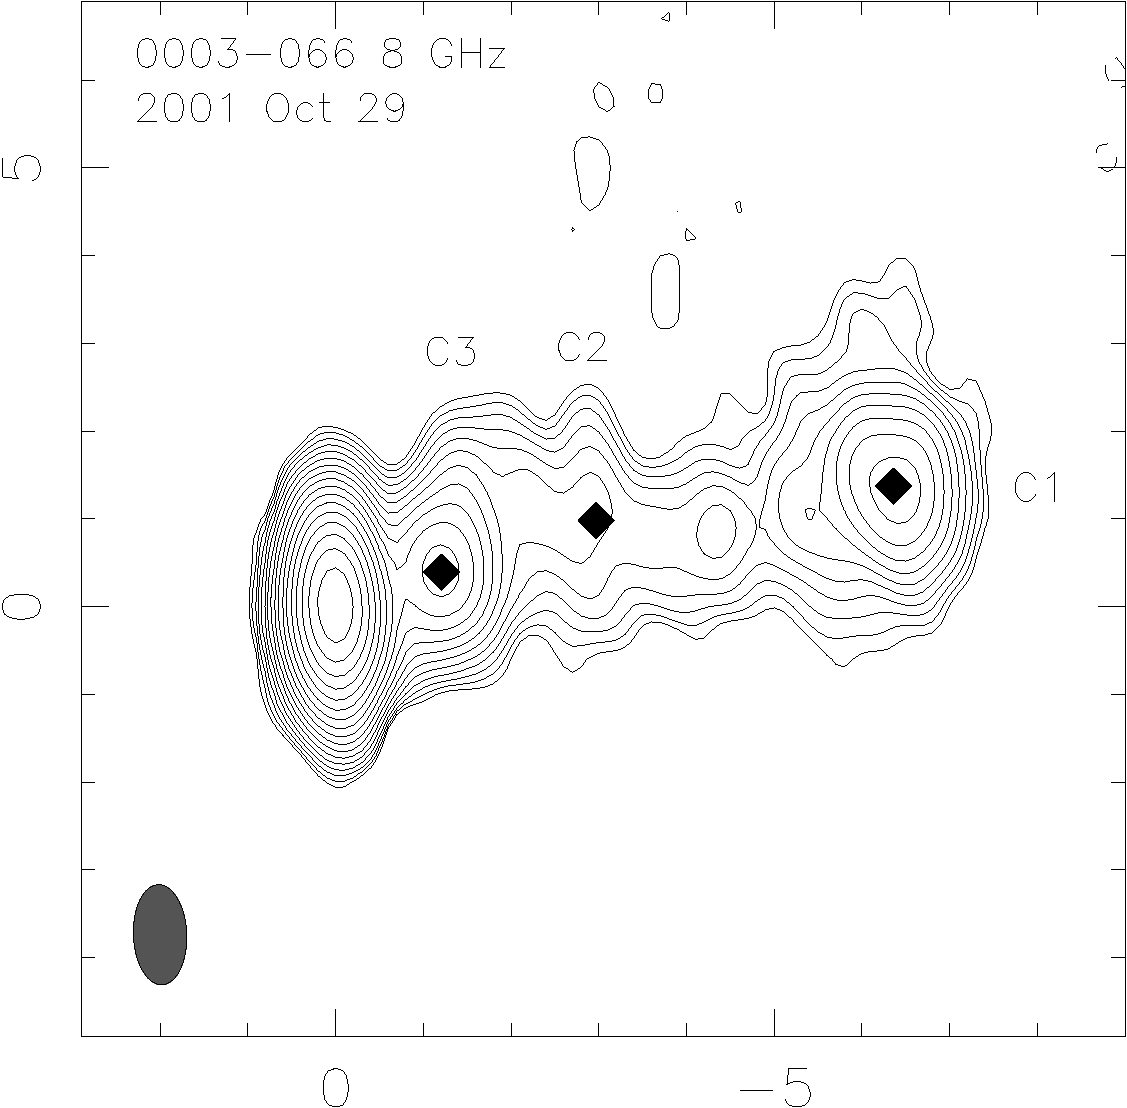
\includegraphics[width=0.7\textwidth]{rdv_0003-066.pdf}
 }
 \caption{Изображение 0003\textminus066 от 29 октября 2001 года из RDV30. По осям отложены
миллисекунды дуги. Самый низкий контур имеет уровень в три раза превышающий уровень шума
\SI{0.9}{\milli\jansky\per\beam}, и каждый последующий контур в корень из двух раз больше. Пиковая
плотность потока составляет \SI{0.96}{\jansky\per\beam}. Размер диаграммы направленности
равен 1.14 на \SI{0.61}{\mas} при позиционном угле \ang{2.3} и показан в
левом нижнем углу изображения. Три залитых ромба указывают на детали струи, которые следовали
модели Гаусса. Параметры гауссовых моделей приведены в таблице~\ref{tab:rdv_mfit}.}
 \label{fig:0003}
\end{figure}

После самокалибровки и построения изображений к видностям, ассоциированным с каждым изображением,
подгонялись Гауссовы модели с помощью задачи \emph{modelfit} в DIFMAP. Такие модели Гауссовы
обеспечивают лаконичное математическое описание положения и свойств различных компонентов
струи на каждом изображении. Подгонка модели в плоскости видимости по сравнению с плоскостью
изображения позволяет достичь разрешения лучше диаграммы направленности в случаях высокого
отношения сигнал/шум; см. также обсуждение подгонки модели в плоскости видностей по сравнению с
подгонкой в плоскости изображения в \cite{Lister_2009b} и предела разрешения в плоскости видности
в \cite{Kovalev_2005}.

Наша процедура подгонки модели была подробно описана в \cite{Piner_2007}, но мы рассмотрим и
суммируем ее здесь. Точное количество используемых гауссовых компонентов и выбор между
эллиптическими или круговыми гауссианами могут быть субъективными, но в данном случае мы исходили из
простоты полученной модели и согласованности модели для данного источника от эпохи к эпохе.
Эллиптические компоненты использовались редко, и только для ядра или яркого компонента струи, когда
остатки, оставшиеся от круговой гауссовой подгонки, были настолько велики, что препятствовали
дальнейшей подгонке модели с использованием карты невязок. Чтобы сохранить последовательность от
эпохи к эпохе, финальная модель из предыдущей или более поздней эпохи часто использовалась в
качестве нулевого приближения для рассматриваемой эпохи. Изредка некоторые подгонки модели из
\cite{Piner_2007} переделывались для согласованности с более поздними эпохами. Подгруппа источников
была смоделирована независимо несколькими авторами для проверки согласованности результатов, и были
получены согласованные результаты кинематики разными моделерами в подавляющем большинстве
($\sim$95\%) случаев. Однако, несмотря на все меры предосторожности, подгонки РСДБ модели не
являются уникальными и представляют только одну математически возможную деконволюцию сложной
структуры источника (см., например, сравнение результатов RDV и 2-см обзора из статьи
\cite{Piner_2007}).

\begin{table}[]
\caption{Гауссовы модели}
\label{tab:rdv_mfit}
\centering
\tiny
\begin{SingleSpace}
\begin{tabular}{l S S S S S S S S S S S S}
\toprule
Источник & {$S$} & {$r$} & {P.A.} & {$a$} & {$(b/a)$} & {P.A.$_\text{maj}$} & Тип & Эпоха &
Компонент & {$a_\text{beam}$} & {$b_\text{beam}$} & {$\theta_\text{beam}$} \\
 & {(\si{\jansky})} & {(\si{\mas})} & {(\si{\degree})}
& {(\si{\mas})} &  & {(\si{\degree})} &  &  &  & {(\si{\mas})} & {(\si{\mas})} & {(\si{\mas})} \\
\multicolumn{1}{c}{(1)} & {(2)} & {(3)} & {(4)} & {(5)} & {(6)} & {(7)} & {(8)} & {(9)} & {(10)} &
{(11)} & {(12)} & {(13)} \\
\midrule
0003\textminus066 & 1.599 & 0.079 &   148.3 & 0.633 & 0.387 & -16.3 & 1 & 1995.78 &  0 &
2.29 & 0.95 & -1.1 \\
           & 0.645 & 1.040 & -60.5 & 1.384 & 1.000 &     0.0 & 1 &         & 99 &      &
  &    \\
           & 0.156 & 5.145 & -74.5 & 3.222 & 1.000 &     0.0 & 1 &         &  1 &      &
  &    \\
           & 1.209 & 0.032 & 114.2 & 0.529 & 0.000 &    21.2 & 1 & 1997.08 &  0 & 2.03 & 0.75 &
-5.8 \\
           & 0.225 & 0.786 & -48.9 & 0.520 & 1.000 &     0.0 & 1 &         &  3 &      &
  &    \\
           & 0.194 & 2.131 & -71.1 & 1.416 & 1.000 &     0.0 & 1 &         &  2 &      &
  &    \\
           & 0.083 & 5.586 & -75.2 & 2.455 & 1.000 &     0.0 & 1 &         &  1 &      &
  &    \\
\bottomrule
\end{tabular}
\end{SingleSpace}

\textbf{Примечания.}
Колонка 1: имя источника B1950.
Колонка 2: плотность потока в Янских.
Колонки 3 and 4: $r$ and P.A. (позиционный угол)~"---полярные координаты центра Гауссианы.
Позиционный угол отсчитывается от севера на восток.
Колонки 5--7: $a$ и $b$~"--- это ширина на половине максимума (FWHM) большой и малой оси Гауссианы,
а P.A.$_\text{maj}$~"--- позиционный угол большой оси. Для круглых компонентов $(b/a)$ и
P.A.$_\text{maj}$ равны 1.0 и 0.0 соответственно.
Колонка 8: тип компонента для команды <<modelfit>> из DIFMAP. Тип 1 обозначает гауссовый компонент.
Тип 0~"--- дельта-функцию.
Колонка 9: эпоха наблюдения.
Компонент 10: номер компонента. Компонент <<0>> обозначает предполагаемое ядро. Остальные
компоненты пронумерованы от 1 до 11, от внешних к внутренним. Номер <<99>> обозначает компонент,
которые не используется в анализе.
Колонки 11--13: $a_\text{beam}$, $b_\text{beam}$ и $\theta_\text{beam}$ --- это FWHM большой оси,
FWHM малой оси и позиционный угол большой оси диаграммы направленности при натуральном взвешивании
(uvweight 0,\textminus1~в DIFMAP).
\end{table}

Полные результаты подбора гауссовой модели представлены в машиночитаемой форме в
таблице~\ref{tab:rdv_mfit}. Таблица~\ref{tab:rdv_mfit} содержит в общей сложности 8571 гауссовых
компонентов, подогнанных к 2753 изображениям, или в среднем около 3 компонентов на изображение (ядро
и два компонента струи). Столбцы 2--8 таблицы~\ref{tab:rdv_mfit} непосредственно соответствуют
результатам работы \emph{modelfit} из DIFMAP и подходят для непосредственного считывания в DIFMAP с
помощью команды \emph{rmodel}. Положение компонентов в Таблице~\ref{tab:rdv_mfit} не были смещены,
чтобы поместить ядро в начало координат, так что положения в Таблице 3 непосредственно соответствуют
позициям на общедоступных изображениях. Обратите внимание, что измерения плотности потока в столбце
2 не очень точны в случае относительно близко расположенных компонентов, где разделение плотности
потока между компонентами может быть неоднозначным.

После после моделирования всех эпох данного источника, компоненты струи должны были быть перекрестно
идентифицированы от эпохи к эпохе, чтобы изучить их кинематику. Эта идентификация компонента
приведена в столбце 10 таблицы~\ref{tab:rdv_mfit}. Компонент <<0>> указывает на предполагаемое ядро.
Другие компоненты пронумерованы от 1 до 11, от самого внешнего компонента внутрь. Идентификатор
компонента <<99>> указывает на неопознанный компонент, не использованный в анализе. Мы
идентифицируем ядро ​​в каждом источнике как компактный компонент в конце структуры односторонней
струи "--- часто, но не всегда, это также самый яркий компонент. Как отмечалось выше, мы исключили
источники, которые, как известно, показывают двусторонние РСДБ структуры на этих масштабах.
Идентификация компонентов струи была сделана на основе согласованности потока, расстояния,
позиционного угла и размера от эпохи к эпохе. Ожидается, что при таком большом количестве эпох на
источник, которые используются здесь, и близком интервале времени, такая идентификация будет
надежной. В тех случаях, когда компонент модели не мог быть непосредственно идентифицирован с
компонентами модели, замеченными в другие эпохи, ему присваивался номер <<99>> в
таблице~\ref{tab:rdv_mfit}, чтобы пометить его как компонент модели, не используемый в анализе. Это
обычно происходило, когда на изображении с несколько более низким разрешением смешивалось вместе то,
что рассматривалось как два отдельных компонента в других моделях (<<слияние>>), или когда компонент
с низким динамическим диапазоном был обнаружен только в нескольких изображениях с плохо ограниченным
положением.

Некоторые общие статистические данные по подгонкам в таблице~\ref{tab:rdv_mfit} приведены ниже. Из
общего числа 8571 компонента 2753 являются ядрами, а 5818~"--- компонентами струи. Около 84\,\%
компонентов (7205) являются круговыми гауссианами, в то время как около 16\% (1366)~"---
эллиптическими. Из 1366 эллиптических гауссианов 1277 (около 93\%) были использованы для
моделирования ядра, в то время как только 89 (около 7\%) использовались для моделирования
компонентов струи. Это означает, что около 46\% компонентов ядра представлены эллипсами, в то время
как только около 2\% компонентов струи представлены эллипсами. Когда ядро ​​моделируется
эллиптическим компонентом, то угол положения большой оси имеет тенденцию выравниваться с углом
положения струи, как показано на рисунке~\ref{fig:rdv_pos_ang_diff}. На этом рисунке показана
гистограмма разницы между углом положения большой оси эллиптического ядра и позиционным углом
ближайшего компонента струи, для 1125 эллиптических ядер с последующим компонентом струи,
смоделированным в ту же эпоху. Избыток при небольших смещениях очевиден, что позволяет предположить,
что эллиптические компоненты ядра моделируют начало структуры удлиненной струи. Аналогичный
результат был найден для компонентов эллиптического ядра для обзора 2 см \cite{Kovalev_2005}.

\begin{figure}[]
 \centerfloat{
  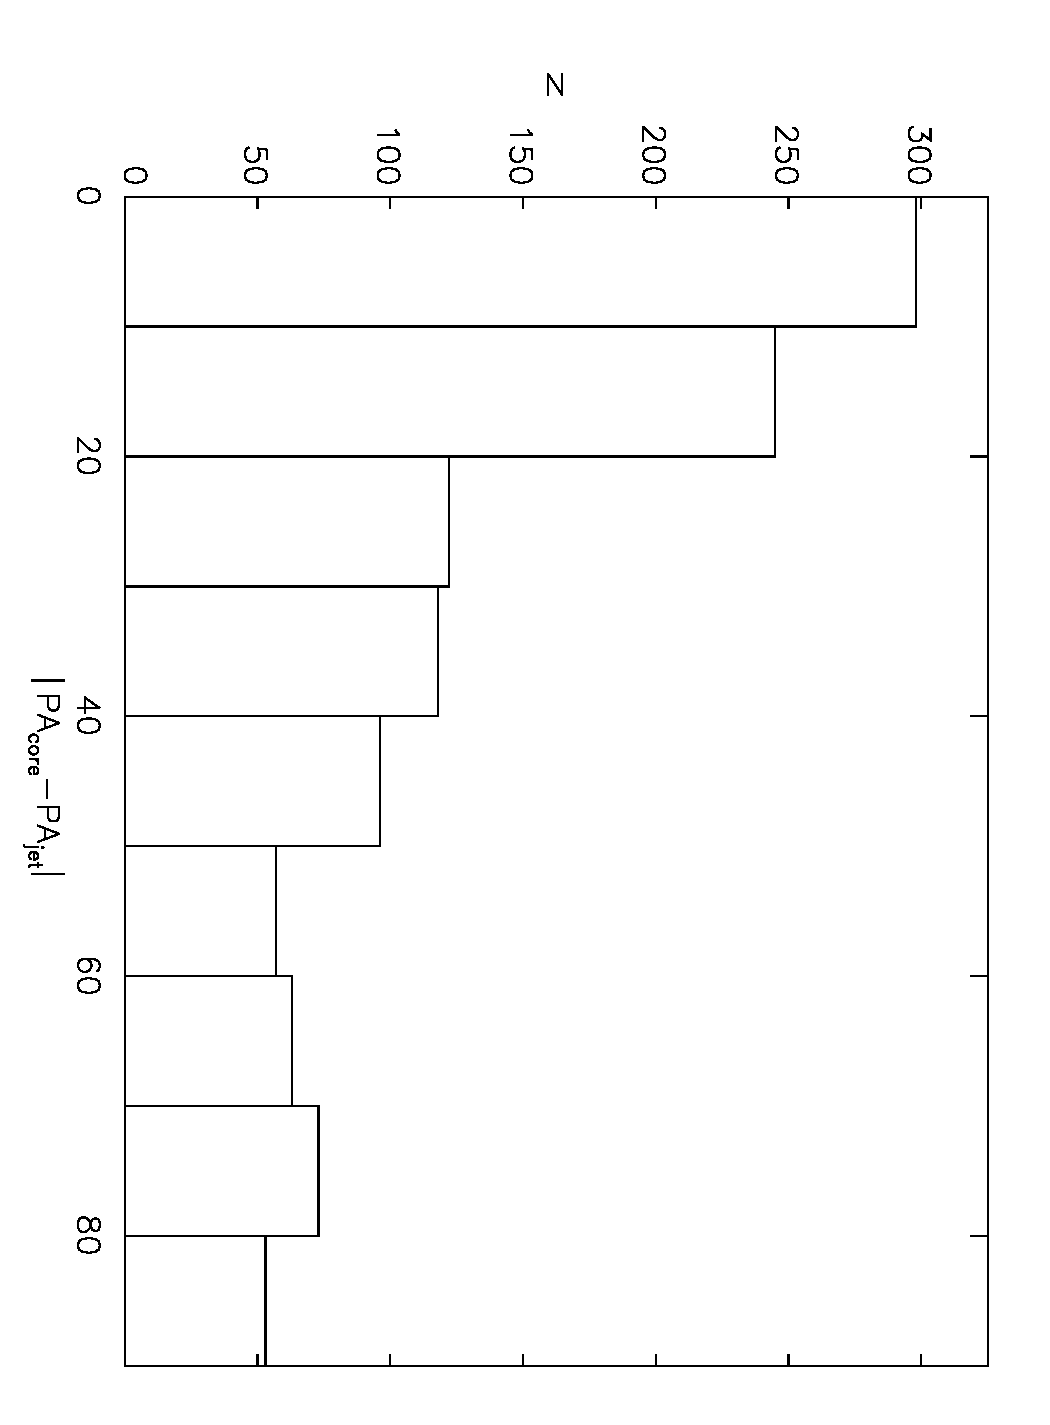
\includegraphics[width=0.7\textwidth,angle=90]{rdv_pos_ang_diff.pdf}
 }
 \caption{Гистограмма разности между позиционным углом большой оси эллиптического ядра
и позиционными углом ближайшего компонента струи, расположенного ниже по потоку.}
 \label{fig:rdv_pos_ang_diff}
\end{figure}

Из 5818 компонентов струи в таблице~\ref{tab:rdv_mfit} 5069 (около 87\,\%) были идентифицированы с
определенным идентификатором компонента в столбце 10 таблицы~\ref{tab:rdv_mfit}, в то время как 749
(около 13\,\%) не идентифицированы (идентификатор <<99>> в столбце 10). Всего имеется 225 уникальных
компонентов струи, по крайней мере, с четырьмя эпохами наблюдения (которые нам необходимы для
кинематического анализа), идентифицированных в 66 источниках в таблице~\ref{tab:rdv_mfit}. При 5069
общих наблюдениях идентифицированных компонентов струи это дает в среднем около 23 наблюдений
каждого из 225 уникальных компонентов.

\begin{table}
\caption{Сравнение обзоров MOJAVE и RDV}
\label{tab:rdv_comptab}
\small
\centering
\begin{tabular}{l c c}
\toprule
Показатель & MOJAVE$^{a}$ & RDV \\
\midrule
Общее количество источников                             & 135  & 68   \\
Количество источников в собственным движением           & 127  & 66   \\
Общее количество изображений                            & 2424 & 2753 \\
%Median number of images per source              & 15   & 43   \\
%Minimum number of images per source             & 5    & 20   \\
Общая продолжительность обзора (годы)                   & 13   & 10   \\
Средний промежуток между изображениями источника (годы) & 0.7  & 0.2  \\
Количество компонентов                                  & 526  & 225  \\
\bottomrule
\end{tabular}

\textbf{Примечания.}
$a$: Использованы опубликованные изображения и кинематика из обзора
MOJAVE~\cite{Lister_2009a,Lister_2009b}.
\end{table}

В таблице~\ref{tab:rdv_comptab} показано сравнение некоторых важных свойств обзора RDV по сравнению
с обзором MOJAVE, опубликованным \cite{Lister_2009a,Lister_2009b}. В то время как общее количество
изображений одинаково для двух обзоров, в обзоре MOJAVE было изучено примерно вдвое больше
источников, и общее количество компонентов примерно в два раза больше, чем в обзоре RDV. Тем не
менее, обзор RDV имеет более высокое среднее число изображений на источник и меньший средний
временной промежуток между изображениями, что полезно для изучения кинематики струи, включая анализ
ускорения.


\subsection{Видимые скорости}

\subsubsection{Методы подгонки}

Мы провели два типа подгонки к каждому из 225 данных о положении компонентов во времени, чтобы
изучить кинематику струи. Первая подгонка была линейной подгонкой $r$ от $t$ с двумя свободными
параметрами. Эти подгонки дают собственное движение как скорость изменения $r$, равную наклону
линии наилучшего соответствия на графике расстояния от времени, и они позволяют проводить прямое
сравнение с измерениями видимой скорости из статьи \cite{Piner_2007}.

Второй тип подгонки был полином второго порядка для $x(t)$ и $y(t)$ отдельно для каждого компонента
и предоставляет информацию о кажущемся ускорении каждого компонента. Используемый здесь метод
нелинейной аппроксимации идентичен методу, описанному \cite{Homan_2001}, а затем использовался в
измерениях ускорения в обзоре MOJAVE \cite{Lister_2009b,Homan_2009}. Мы используем ту же
параметризацию для подгонки, что и \cite{Homan_2001} и \cite{Homan_2009}, что позволяет проводить
прямое сравнение наших результатов с результатами ускорения в MOJAVE. Мы суммируем этот нелинейный
метод подгонки ниже.

В этих нелинейных подгонках используются три параметра для $x(t)$ и $y(t)$, т.\:е. в общей
сложности шесть свободных параметров для каждого компонента. Вектор собственного движения
для каждой подгонки определяется из среднего собственного движения в направлениях $x$ и $y$
($\mu_x$ и $\mu_y$) или, что эквивалентно, вектора собственного движения в середине времени
$t_\text{mid} = (t_i + t_f) / 2$, где $t_i$ и $t_f$~"--- времена начального и конечного наблюдения
компонента, соответственно. Величина среднего вектора собственного движения
обозначается $\mu$, а направление этого вектора~"--- $\phi$. Величина $\mu$ затем преобразуется в
наблюдаемую кажущуюся скорость $\beta_\text{app}$. Величина $|\text{P.A.} - \phi|$ дает разность
между средневзвешенным позиционным углом P.A. компонента и направлением вектора его средней видимой
скорости.

Кажущееся угловое ускорение вычисляется из $\ddot{x}$ и $\ddot{y}$ ($\dot{\mu}_x$ и $\dot{\mu}_y$).
Это кажущееся угловое ускорение раскладывается на две составляющие, параллельные и перпендикулярные
направлению номинальной скорости $\phi$. Эти два компонента обозначены $\dot{\mu}_{\parallel}$ и
$\dot{\mu}_{\perp}$, и они представляют кажущееся угловое ускорение из-за изменений в кажущейся
скорости и из-за изменений направления, соответственно. Чтобы легче было сравнивать кажущиеся
ускорения среди высокоскоростных и низкоскоростных джетов, относительное параллельное ускорение
определяется как
\begin{equation}
\label{eq:rdv_relpar}
\dot{\eta}_{\parallel}\equiv
\dot{\beta}_\mathrm{\parallel app}/\beta_\mathrm{app}=(1+z)\dot{\mu}_{\parallel}/\mu\,,
\end{equation}
а относительное перпендикулярное ускорение определяется как
\begin{equation}
\label{eq:rdv_relperp}
\dot{\eta}_{\perp}\equiv
\dot{\beta}_\mathrm{\perp app}/\beta_\mathrm{app}=(1+z)\dot{\mu}_{\perp}/\mu\,.
\end{equation}
Таким образом, компонент с относительным параллельным ускорением 0.1, например, имеет кажущуюся
скорость, которая увеличивается на 10\,\% в год. Отметим также, что относительное ускорение,
определенное таким образом, имеет размерность обратного времени. Эти подгонки предполагают
постоянное ускорение в течение времени наблюдения за компонентом, хотя мы не можем исключать
возможность того, что более сложные и переменные во времени ускорения также могут иметь место.

Для обоих методов подгонки (линейного и нелинейного) ошибки в измерениях положения были определены
в соответствии с методом, описанным в \cite{Homan_2001} и впоследствии используется в
\cite{Lister_2009b,Homan_2009}. Этот метод использует разброс точек вокруг подгонки, чтобы
назначить постоянную погрешность для каждой точки, такой что значение $\chi^{2}$
подгонки имело значение 1.0. Это отличается от метода на основе диаграммы направленности для
назначения позиционных ошибок, который мы использовали в статье \cite{Piner_2007}. Новый метод
имеет тот недостаток, что значение $\chi^{2}$ нельзя использовать для определения пригодности
выбранной модели, но при условии, что модель уместно, это дает хорошие неопределенности для
параметров модели. В нем также прямо рассматривается хорошо известная проблема в РСДБ моделировании,
которая заключается в том, что при большом количестве измерений положения не существует метода для
получения надежных и статистически точных неопределенностей, которые будут работать для всех
компонентов в наборе данных, и будут приняты во внимание как ошибки, вызванные погрешностями
измерений видности, так и систематические эффекты, вызванные изменениями в количестве и форме
компонентов модели, или эффектами, введенными во время калибровки и построения изображений.

Результаты линейных подгонок представлены в Таблице 5 и показаны в виде графиков расстояния в
зависимости от времени на Рисунке 3. Таблица 5 этого документа аналогична Таблице 4 в
\cite{Piner_2007}, но в этой статье в среднем примерно в четыре раза больше точек на
компонент, чем в \cite{Piner_2007}. Таким образом, мы опустили <<Код качества>>,
который мы связали с каждым компонентом в \cite{Piner_2007}, поскольку в данной работе практически
все фиты соответствуют качеству <<хорошо>> или <<отлично>>, как определено в той статье. В таблице
5 приведены средняя плотность потока и средневзвешенное расстояние каждого компонента, собственное
радиальное движение и видимая скорость, а также экстраполированная эпоха, когда компонент отделился
от ядра, для компонентов, которые имеют значимость собственного движения выше $3\sigma$. Полный
набор из 66 графиков на рисунке 3 доступен в онлайн-версии журнала. Линейные подгонки в таблице
5 представлены в основном для соответствия с \cite{Piner_2007}; однако, большая часть
последующего анализа в этой статье использует результаты нелинейных подгонок из таблицы 6.

Результаты нелинейной подгонки для каждого из 225 компонентов представлены в таблице 6 и графически
показаны на рисунке 4 в виде полиномов второго порядка как $x(t)$, так и $y(t)$ для
каждого компонента в Таблица 6. Полный набор из 225 графиков на рисунке 4 доступен в
онлайн-версии журнала. Обратите внимание, что в колонках 9--14 таблицы 6 не приводятся никакие
записи, если погрешность направления движения >\,\ang{90}. Обычно это происходит
из-за компонентов, которые почти неподвижны, так что направление движения и, следовательно, все
последующие столбцы, которые зависят от направления движения, не определены. Заголовки столбцов в
Таблице 6 идентичны заголовкам в соответствующей таблице в \cite{Homan_2009} (Таблица 1), чтобы
помочь в сравнении между двумя анализами ускорения. Одно из основных отличий между таблицей 6 и
соответствующей таблицей из \cite{Homan_2009} состоит в том, что в таблице 1 из \cite{Homan_2009}
показан анализ ускорения только для высококачественной подвыборки из 203 компонентов, которые
удовлетворяют определенным критериям отбора, из 526 всех компонентов в обзоре MOJAVE. В этой статье
в Таблице 6 представлены подгонки второго порядка для всех 225 компонентов в обзоре RDV, а затем
мы вводим отсечку по качеству данных, аналогичные тем, которые были введены \cite{Homan_2009},
прежде чем проводить анализ ускорения в Разделе 5.

\subsubsection{Изменения скорости в источниках}

На рисунке 5 показана гистограмма измеренной видимой величины скорости $\beta_\text{app}$ из
таблицы 6 для всех компонентов из таблицы 6 ($N = 224$ для 65 источников с красным смещением;
1657\textminus261 не имеет измеренного красного смещения). Средняя кажущаяся скорость компонента на
рисунке 5 составляет $7.2 c$, а медианная кажущаяся скорость равна $4.5 c$. Здесь мы обсудим
изменение кажущейся скорости от компонента к компоненту в отдельных источниках, а затем обсудим
видимые изменения скорости среди разных источников в следующем подразделе.

В целом, мы подтверждаем общую тенденцию, наблюдаемую в других исследованиях распределений видимых
скоростей: что, хотя подавляющее большинство компонентов движется наружу, существует также
небольшое, но не пренебрежимо малое количество, по-видимому, движущихся внутрь компонентов и почти
неподвижных компонентов \cite{Lister_2009b,Britzen_2008}. В обзоре RDV 185 из 218 компонентов в
Таблице 6 с измеренным значением $|\text{P.A.} - \phi |$ движутся <<наружу>> ($|\text{P.A.} -
\phi|\leqslant \ang{90}$), в то время как только 33 движутся <<внутрь>> ($|\text{P.A.} - \phi| >
\ang{90}$) "--- и большинство из этих 33 измерений не являются статистически значимыми. Только 10 из
этих 33 компонентов движутся внутрь со значимостью $>3\sigma$, все они также имеют отрицательное
измеренное значение их радиальной кажущейся скорости в Таблице 5, как и ожидалось. В
\cite{Lister_2009b} подробно обсуждаются пять различных геометрических эффектов, которые могут
привести к <<иллюзии>> видимого движения внутрь; ни один из них не представляет собой реальное
объемное  движение вещества джета внутрь, и вполне вероятно, что некоторая комбинация этих пяти
эффектов действует на это небольшое подмножество компонентов здесь.

Мы также подтверждаем существование подмножества медленно движущихся или почти неподвижных (Low
Pattern Speed или LPS) компонентов с тем же количеством и расстояниями от ядра, как было
обнаружено в обзоре MOJAVE \cite{Lister_2009b}. В Таблице 6 всего 43 компонента с собственным
движением менее \SI{50}{\uas\per\year}, что является ограничением собственного движения для
компонента LPS в \cite{Lister_2009b}. Из этих 43, 21 также соответствуют двум другим критериям для
компонента LPS, используемого \cite{Lister_2009b}: нет значительного ускорения и скорость
значительно ниже, чем у других компонентов в той же струе. Здесь мы количественно определяем эти два
критерия, так значения $\dot{\eta}_{\parallel}$ и $\dot{\eta}_{\perp}$ должно быть меньше
$2\sigma$, а значение $\beta_\text{app}$ меньше, чем средневзвешенное значение $\beta_\text{app}$
для других компонентов в струе, по крайней мере, на $2\sigma$. 21 компонент в 19 источниках,
которые соответствуют всем трем из этих критериев, отмечены как компоненты LPS в Таблице 6.

С этими критериями компоненты LPS составляют около 9\,\% от компонентов струи в обзоре RDV, и мы
обнаруживаем, что эти компоненты LPS находятся ближе к ядру, чем общая популяция компонентов струи.
Более половины (12 из 21) компонентов LPS сгруппированы на проекционных расстояниях
$\sim\SI{4}{\parsec}$ от ядра (а остальные 9 разбросаны до проецируемых расстояний
$\sim\SI{40}{\parsec}$), в то время как медианная проекция расстояние от ядра для не-LPS
компонентов  составляет \SI{9}{\parsec}. В 8 из 19 источников с компонентами LPS компонент LPS
является ближайшим к ядру. Для сравнения, \cite{Lister_2009b} обнаружили, что общая частота
встречаемости составляет около 6\,\% (31 из 526 компонентов), а типичная проекция расстояния
до ядра составляют менее \SI{9}{\parsec} для компонентов LPS. Такие, по-видимому, стационарные
детали могут быть вызваны проекционными эффектами, если струя проходит очень близко к лучу зрения,
или они могут быть внутренне стационарными деталями, такими как устойчивые реколлимационные
ударные волны, которые ожидаются при моделировании струи (например, \cite{Gomez_1995}), и это может
иметь тенденцию происходить на одинаковых расстояниях от ядра. Тогда в обзоре RDV около 1/6
источников (12 из 66) имеют то, что можно интерпретировать как стационарную деталь, такую ​​как
реколлимационный шок в проекции расстояния $\sim\SI{4}{\parsec}$ от ядра (несколько десятков
парсек de-projected для ожидаемых малых углов обзора). Из 21 LPS компонента 20 находятся в
квазарах, 1~"--- в галактике, и ни один не находится в объектах BL\,Lac, основываясь на оптических
идентификациях в Таблице~\ref{tab:rdv_sources}. В то время как \cite{Lister_2009b} обнаруживает, что
частота появления LPS объектов выше в их объектах BL\,Lac, отметим, что в выборке RDV имеется
только 7 объектов BL\,Lac.

Если струи в обзоре RDV в среднем ускоряются или замедляются, то можно ожидать, что будет
наблюдаться постоянное ощущение изменения измеренных видимых скоростей от компонента к компоненту в
источнике, поскольку компоненты, удаленные от ядра, будут либо систематически быстрее, либо
систематически медленнее, чем компоненты ближе к ядру. Мы исследуем эту связь между кажущейся
скоростью компонентов и средним расстоянием от ядра здесь, а затем исследуем ускоренное движение
отдельных компонентов в Разделе 5. Для каждого из 56 источников в Таблице 6, которые имеют по
крайней мере два нестационарных компонента со значимостью измерении видимой скорости
$\geqslant1\sigma$ мы выполнили подгонку к $\ln \beta_\text{app}$ от $\ln \langle r \rangle$,
используя измеренные значения из таблицы 6 (исключая все кажущиеся скорости со значимостью
$<1\sigma$ и все стационарные компоненты, см. выше). Постоянное положительное видимое ускорение
вдоль струи в источнике дало бы наклон 0.5 для такого фита. На рис. 6 показан пример одной из этих
подгонок (для источника 1514\textminus241 с наклоном 0.5, близким к среднему наклону для всех
подгонок), а на рис. 7 показана гистограмма всех 56 наклонов. Для 56 отдельных подгонок 43 дают
положительный наклон, а 13 подгонок дают отрицательный наклон, при этом средний уклон составляет
0.55 (близко к значению 0.5, ожидаемому для постоянного ускорения в источнике), а медианное
значение составляет 0.34. Биномиальная вероятность измерения 43 положительных уклонов, если они
были случайным образом распределены между положительными и отрицательными значениями, составляет
только $P = \num{4e-5}$. Если мы посчитаем только уклоны, имеющие значимость не менее $2\sigma$,
чтобы мы могли быть уверены в знаке, то мы найдем 22 положительных наклона и 7 отрицательных с
биномиальной вероятностью $P = \num{4e-3}$. Поэтому мы приходим к выводу, что в среднем в нашей
выборке компоненты, находящиеся дальше от ядра, имеют большие кажущиеся скорости, чем компоненты,
расположенные ближе к ядру в данном источнике, с высокой статистической значимостью. Мы обсуждаем
связь этого результата с другими результатами в литературе в разделе 6. Если компоненты дальше от
ядра движутся быстрее, чем более близкие компоненты, то отдельные компоненты должны в среднем
испытывать положительные кажущиеся параллельные ускорения. Мы обсуждаем кажущиеся параллельные
ускорения отдельных компонентов в разделе 5.1.
